\documentclass{article}
\usepackage[hyphens]{url}
\usepackage{mathtools}
\usepackage{amsmath}
\usepackage{listings}
\usepackage{graphicx}
\usepackage[margin=1in]{geometry}
\usepackage{float}
\floatstyle{boxed}
\restylefloat{figure}
\lstset{basicstyle=\footnotesize, breaklines=true}
\begin{document}


\title{CS595 Intro to Web Science, Assignment \#8}
\author{Valentina Neblitt-Jones}
\date{November 14, 2013}
\maketitle



\section*{Instructions}

The goal of this project it is to use the basic recommendation principles we have learned for user-collected data. You will modify the code given to you which performs movie recommendations from the MovieLense data sets. \\

The MovieLense data sets were collected by the GroupLens Research Project at the University of Minnesota during the seven-month period from September 19th, 1997 through April 22, 1998. It is available for download from \url{http://www.grouplens.org/node/73} \\

There are three files which we will use: 

\subsection*{u.data}

u.data: 100,000 ratings by 943 users on 1,682 movies. Each user has rated at least 20 movies. Users and items are numbered consecutively from 1. The data is randomly ordered. This is a tab-separated list of user id, item id, rating, and timestamp. \\

The time stamps are unix seconds since 1/1/1970 UTC. \\

Example: 

\begin{table}[!h]
\centering
\begin{tabular}{c c c c}
user id & item id &  rating & timestamp \\
\hline
196 & 242 & 3 & 881250949 \\
186 & 302 & 3 & 891717742 \\
22 & 377 & 1 & 878887116 \\
244 & 51 & 2 & 880606923 \\
166 & 346 & 1 & 886397596 \\
298 & 474 & 4 & 884182806 \\
115 & 265 & 2 & 881171488 \\
\end{tabular}
\end{table}

\subsection*{u.item}

u.item: Information about the 1,682 movies. This is a tab separated list of movie id, movie title, release date, video release date, IMDb URL, unknown, Action, Adventure, Animation, Children's, Comedy, Crime, Documentary, Drama, Fantasy, Film-Noir, Horror, Musical, Mystery, Romance, Sci-Fi, Thriller, War, and Western. \\

The last 19 fields are the genres, a 1 indicates the movie is of that genre, a 0 indicates it is not; movies can be in several genres at once. The movie ids are the ones used in the u.data set. \\

Example: \\

\begin{table}[!h]
\centering
\begin{tabular}{c c c c c c}
movie id & movie title & release date & video release date & IMDb URL \\
\hline
161 & Top Gun (1986) & 01-Jan-1986 &  & \url{http://us.imdb.com/M/title-exact?Top%20Gun%20(1986)} &(1986) \\
%186 & 302 & 3 & 891717742 \\
%22 & 377 & 1 & 878887116 \\
\end{tabular}
\end{table}

\begin{verbatim}
161|Top Gun (1986)|01-Jan-1986||http://us.imdb.com/M/title-exact?Top\%20Gun\%20(1986)|0|1|0|0|0|0|0|0|0|0|0|0|0|0|1|0|0|0|0 
162|On Golden Pond (1981)|01-Jan-1981||http://us.imdb.com/M/title-exact?On\%20Golden\%20Pond\%20(1981)|0|0|0|0|0|0|0|0|1|0|0|0|0|0|0|0|0|0|0 
163|Return of the Pink Panther, The (1974)|01-Jan-1974||http://us.imdb.com/M/title-exact?Return\%20of\%20the\%20Pink\%20Panther,\%20The\%20(1974)|0|0|0|0|0|1|0|0|0|0|0|0|0|0| 0|0|0|0|0
\end{verbatim}

\subsection*{u.user}

u.user: Demographic information about the users. This is a tab-separate list of user id, age, gender, occupation, and zip code. \\

Example: \\

\begin{table}[!h]
\centering
\begin{tabular}{c c c c c}
user id & age &  gender & occupation & zip code \\
\hline
1 & 24 & M & technician & 85711 \\
2 & 53 & F & other & 94043 \\
2 & 23 & M & writer & 32067 \\
4 & 24 & M & technician & 43537 \\
5 & 33 & F & other & 15213 \\
\end{tabular}
\end{table}

The code for reading from the u.data and u.item files and creating recommendations is described in the book Programming Collective Intelligence (check mail for more details). You are to modify recommendations.py to answer the following questions. Each question your program answers correctly will award you 10 points. You must have the question answered completely correct; partial credit will be only awarded if your answer is very close to the correct one.

\subsection*{Answer to Question 1}

%\begin{lstlisting}[frame=single, caption=index.html, label=webpage]
%\end{lstlisting}

%\begin{figure}[H]
%\centering
%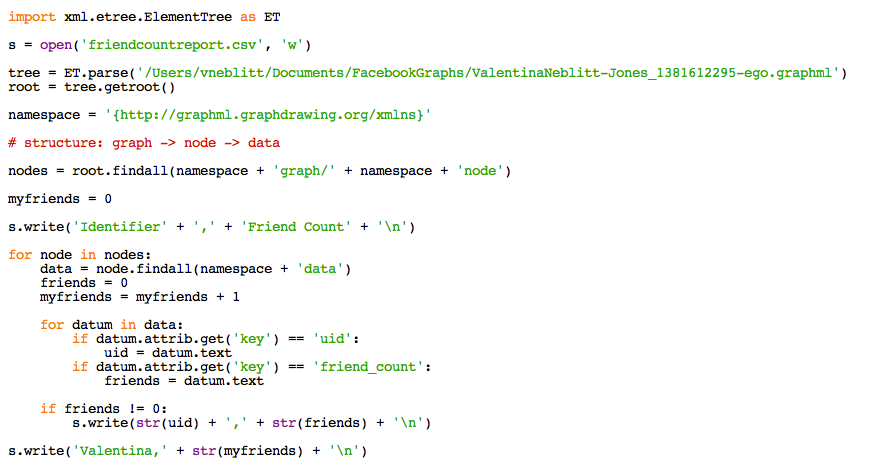
\includegraphics[scale=0.50]{q1/GetFriendCountsCode}
%\caption{Showing Friend Count}
%\label{GetFriendCountsCode}
%\end{figure}

%\begin{table}[!h]
%\centering

%\begin{tabular}{c c c c}
%\hline
%Identifier & Model &  Actual & Hit/Miss \\
%\hline
%\hline
%1 & Mr. Hi & Mr. Hi & Hit \\
%2 & Mr. Hi & Mr. Hi & Hit \\
%3 & Mr. Hi & Mr. Hi & Hit \\
%4 & Mr. Hi & Mr. Hi & Hit \\
%5 & Mr. Hi & Mr. Hi & Hit \\
%6 & Mr. Hi & Mr. Hi & Hit \\
%7 & Mr. Hi & Mr. Hi & Hit \\
%8 & Mr. Hi & Mr. Hi & Hit \\
%9 & Mr. Hi & Mr. Hi & Hit \\
%10 & Mr. Hi & John & Miss \\
%\hline
%\end{tabular}
%\caption{Results of Model vs. Actual}
%\end{table}

\newpage

\section*{Extra Credit, 3 Points}

Use D3 to create a who-follows-whom graph of your Twitter account. Use my Twitter account (phonedude\_mln) if you do not have an interesting number of followers.

%\begin{table}[!h]
%\centering
%\caption{Results of Model vs. Actual}
%\begin{tabular}{c c c c}
%\hline
%Identifier & Model &  Actual & Hit/Miss \\
%\hline
%\hline
%0.150 & 0.014 & Mr. Hi & Hit \\
%0.085 & John & Mr. Hi & Hit \\
%\hline
%\end{tabular}
%\end{table}

\subsection*{Answer to Extra Credit}

Not attempted.



\newpage

\section*{Resources}

Note: Apologies. I did not have time to implement BibTex for this assignment, but I will on Assignments 8, 9, and 10.

%\begin{itemize}
%\item Bostock, Michael. Data-Driven Documents. \url{http://d3js.org/}
%\item Bostock, Michael. Labeled Force Layout. \url{http://bl.ocks.org/mbostock/950642}
%\item Bostock, Michael. Selections. \url{https://github.com/mbostock/d3/wiki/Selections#wiki-on}
%\item Bostock, Michael. mbostock/d3. \url{https://github.com/mbostock/d3}
%\item Bostock, Michael. mbostock/d3: API Reference. \url{https://github.com/mbostock/d3/wiki/API-Reference}
%\item Murray, Scott. About these tutorial. \url{http://alignedleft.com/tutorials/d3/about}
%\item Murray, Scott. Interactive Data Visualization: An Introduction to Designing with D3. Via Safari Books Online
%\item NetworkX developer team. NetworkX. \url{http://networkx.github.io/}
%\item NetworkX developer team. NetworkX: edge\_betweenness\_centrality. \url{http://networkx.github.io/documentation/latest/reference/generated/networkx.algorithms.centrality.edge_betweenness_centrality.html#networkx.algorithms.centrality.edge_betweenness_centrality}
%\item NetworkX developer team. NetworkX: Graph - Undirected graphs with self loops. \url{http://networkx.github.io/documentation/latest/reference/classes.graph.html#networkx.Graph}
%\item NetworkX developer team. NetworkX: node\_link\_data. \url{http://networkx.lanl.gov/reference/generated/networkx.readwrite.json_graph.node_link_data.html#networkx.readwrite.json_graph.node_link_data}
%\item NetworkX developer team. NetworkX: node\_link\_graph. \url{http://networkx.lanl.gov/reference/generated/networkx.readwrite.json_graph.node_link_graph.html#networkx.readwrite.json_graph.node_link_graph}
%\item NetworkX developer team. NetworkX: number\_connected\_components. \url{http://networkx.github.io/documentation/latest/reference/generated/networkx.algorithms.components.connected.number_connected_components.html#networkx.algorithms.components.connected.number_connected_components}
%\item PyMOTW. json: JavaScript Objection Notation Serializer. \url{http://pymotw.com/2/json/}
%\item Python.org. json: JSON encoder and decoder. \url{http://docs.python.org/3.3/library/json.html}
%\item Python.org. print: Data pretty printer. \url{http://docs.python.org/2/library/pprint.html}
%\item Stack Overflow. Parsing values from a JSON file in Python. \url{http://stackoverflow.com/questions/2835559/parsing-values-from-a-json-file-in-python}
%\item Stack Overflow. Skip the first couple of lines while reading lines in Python file. \url{http://stackoverflow.com/questions/9578580/skip-first-couple-of-lines-while-reading-lines-in-python-file}
%\end{itemize}

\end{document}